%!Tex Root = multiRelation.tex

\section{Induced Relational Views}
\label{sec:Induced Relational Views}
In this section, we discuss the notion of induced relational views, which is central to our induced relational GCN framework developed in~\Cref{sec:gcn}. First, in~\Cref{sub:Induced Views}, we introduce potential strategies for selecting the accepted answer to a question. We show how each strategy induces a graph $G$ on the set of all question-answer $(q,a)$ tuples. Next, in~\Cref{sub:Generalized Views}, we show how each of these sample strategies is an instance of an equivalence relation; our framework generalizes to incorporate any such relation.

%we show how each of these example strategies is an instance of a generalized principle; our framework generalizes to incorporate any equivalence relation.




% \label{sec:motivation}
% \begin{figure}[t]
%     \centering
%       %  \includegraphics[scale=0.4]{figures/Contrast}
%     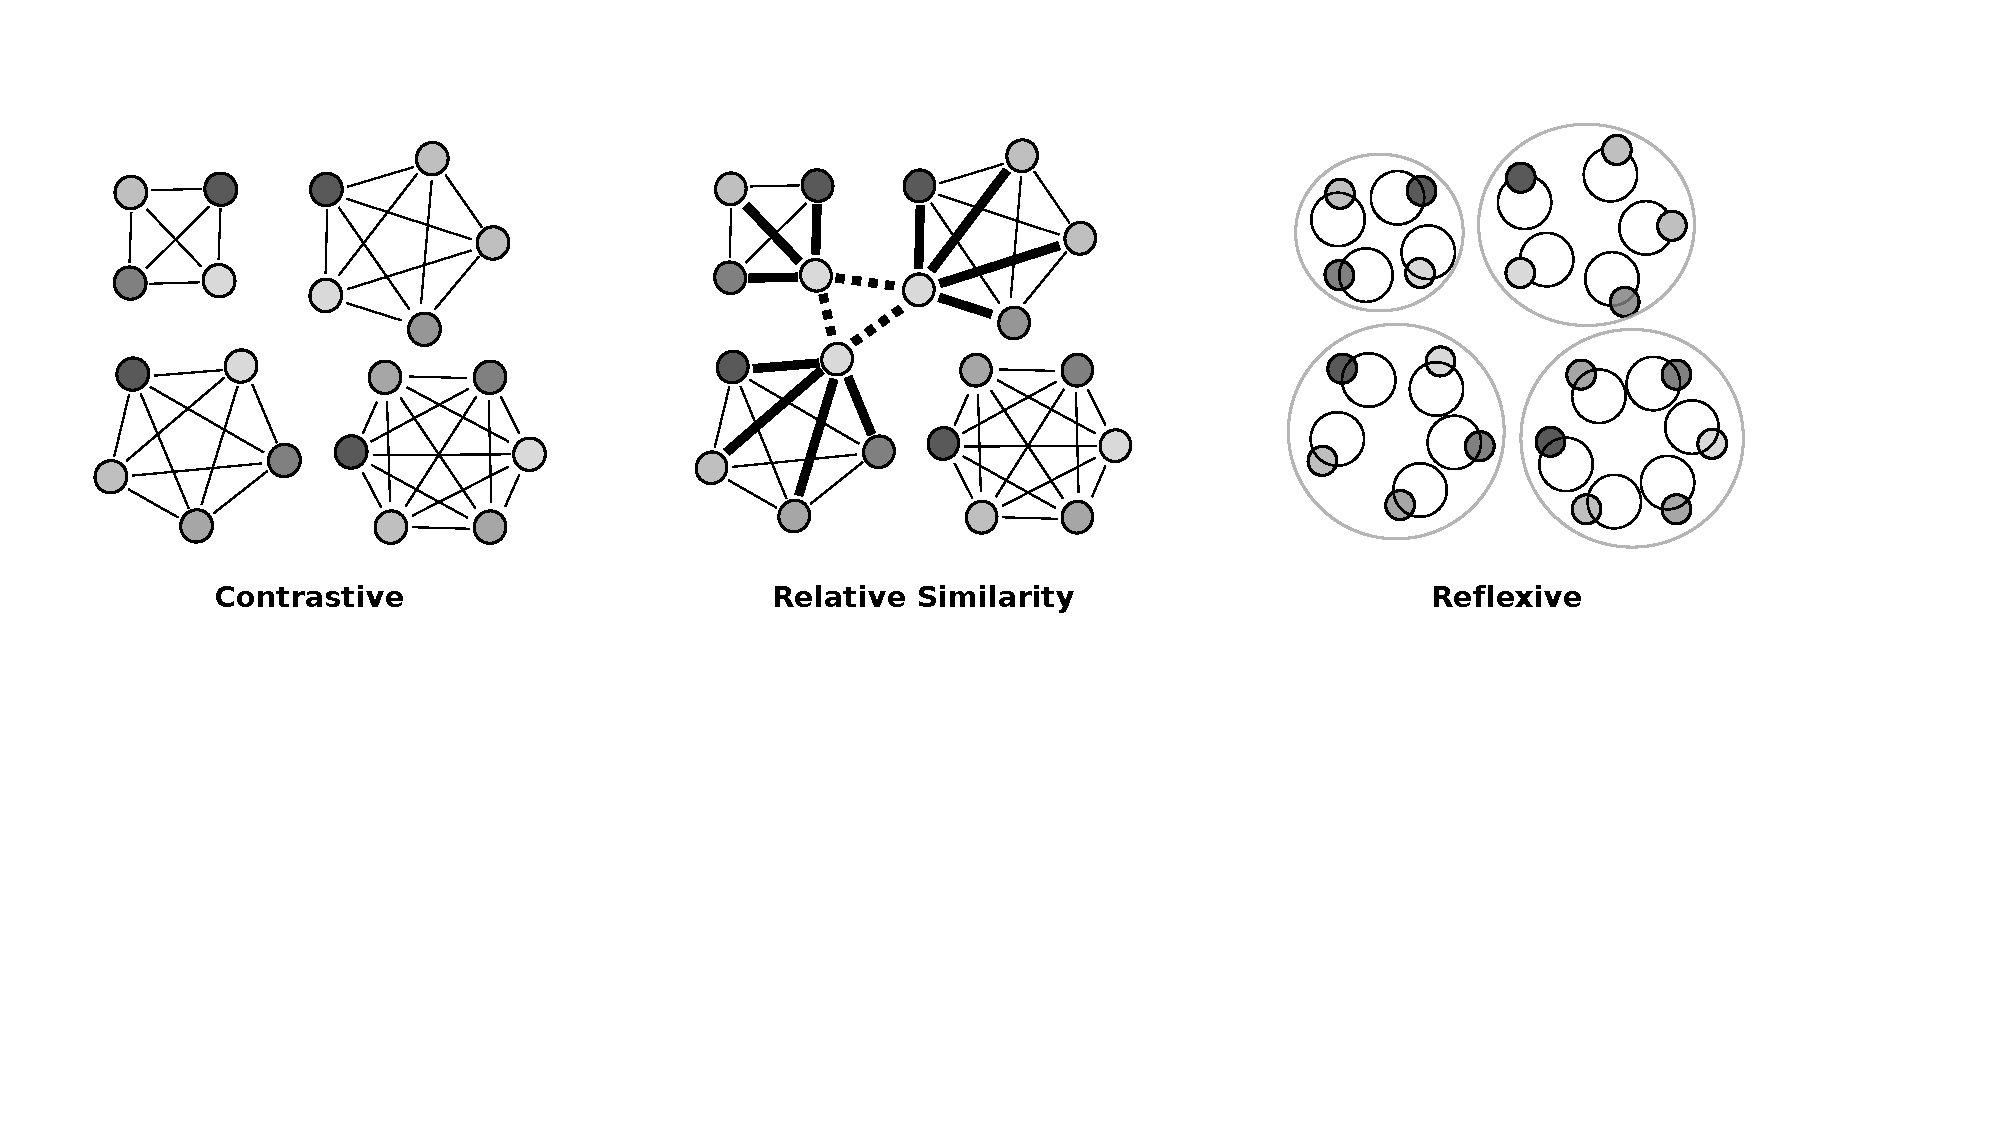
\includegraphics[width=\columnwidth
%     % clip, viewport= 0in 2.65in 12.5in 7.25in
%     ]{figures/Relation}
%         \caption{\small \label{fig:relation} Contrastive, Similarity by contrast and Reflexive strategies among $(q,a)$ tuples. Contrastive strategy is used to compare between all answers to a question;  Similarity by contrast connects answers by the same author across questions if relative difference in author's skill with other answerers in each question are significant. Reflexive assumes no dependence on other answers for prediction. }
%     \vspace{-0.1in}
% \end{figure}
\begin{figure*}[h]
    \centering
    \begin{subfigure}{0.25\textwidth}
        \centering
        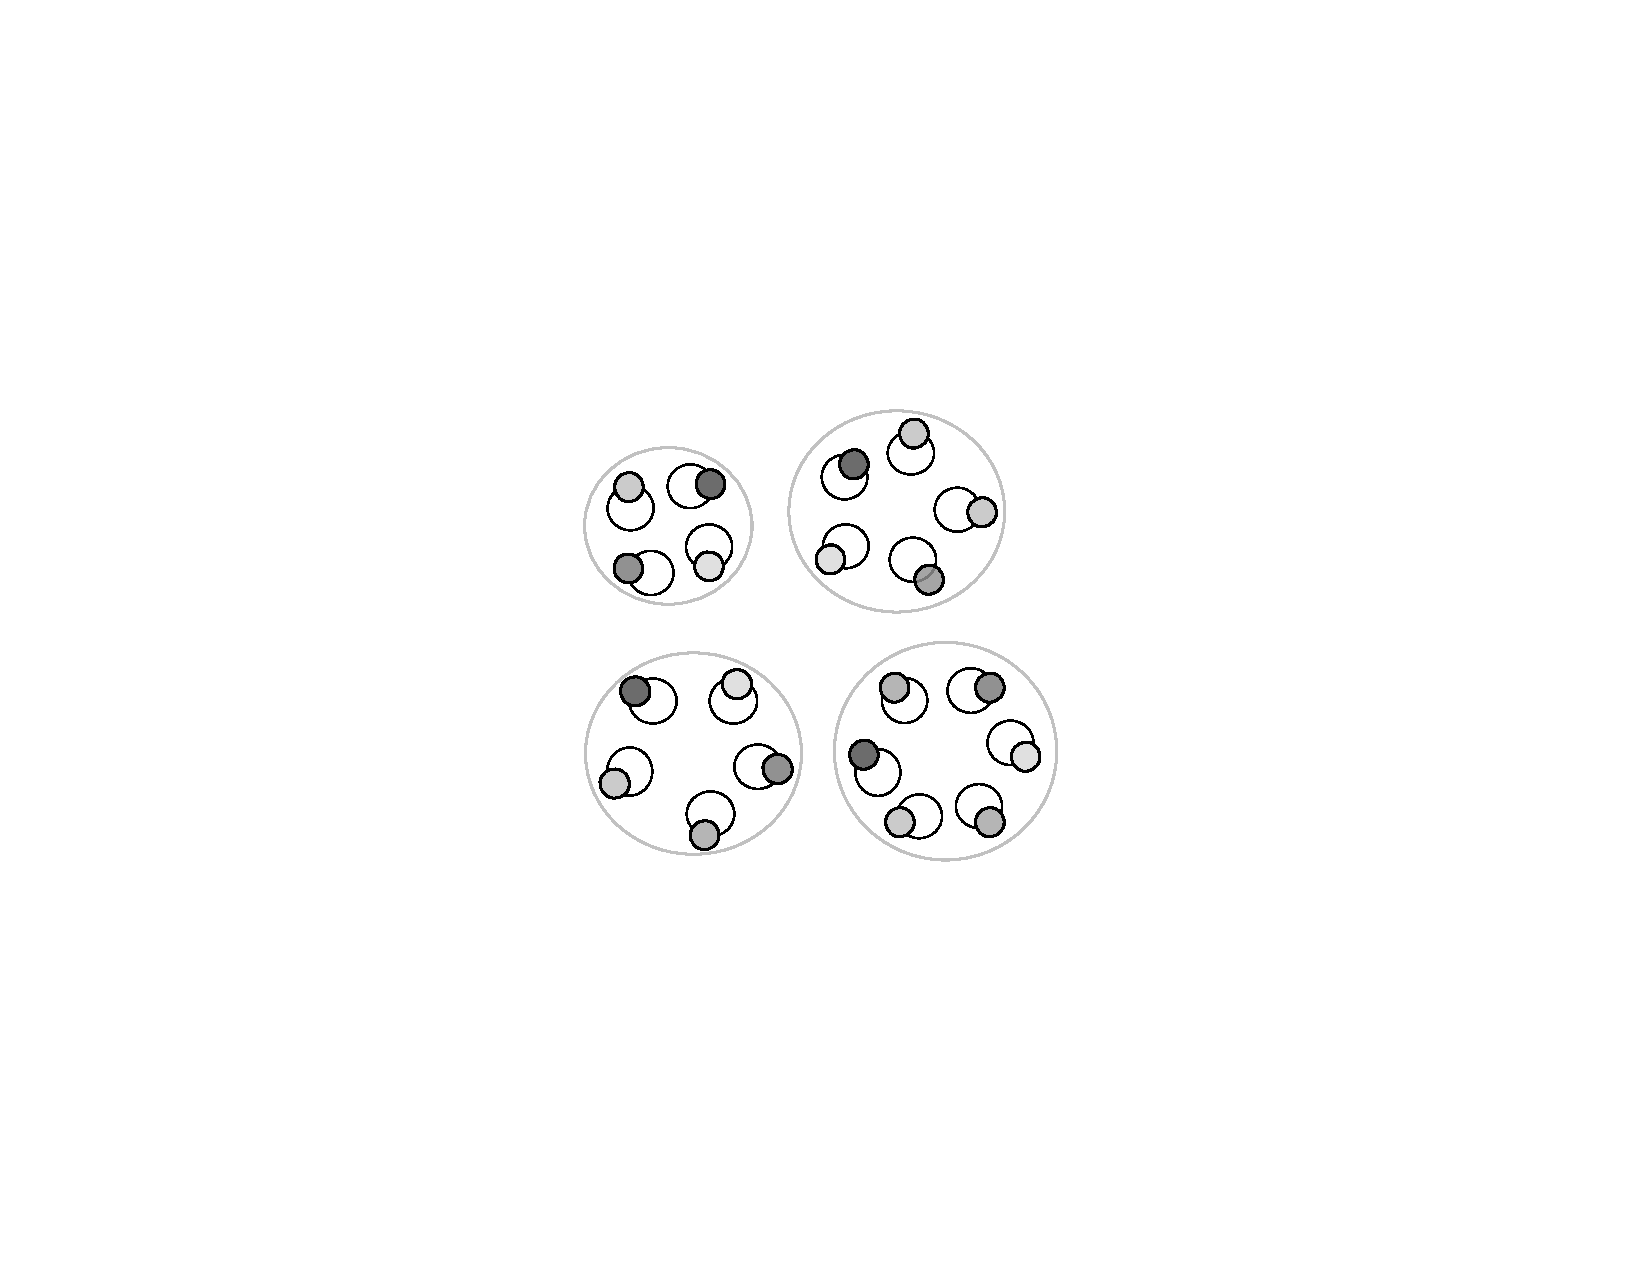
\includegraphics[scale=0.3]{figures/reflex_updated}
            \caption{Reflexive}
            \label{fig:reflexive}
    \end{subfigure}%
    \begin{subfigure}{0.27\textwidth}
        \centering
        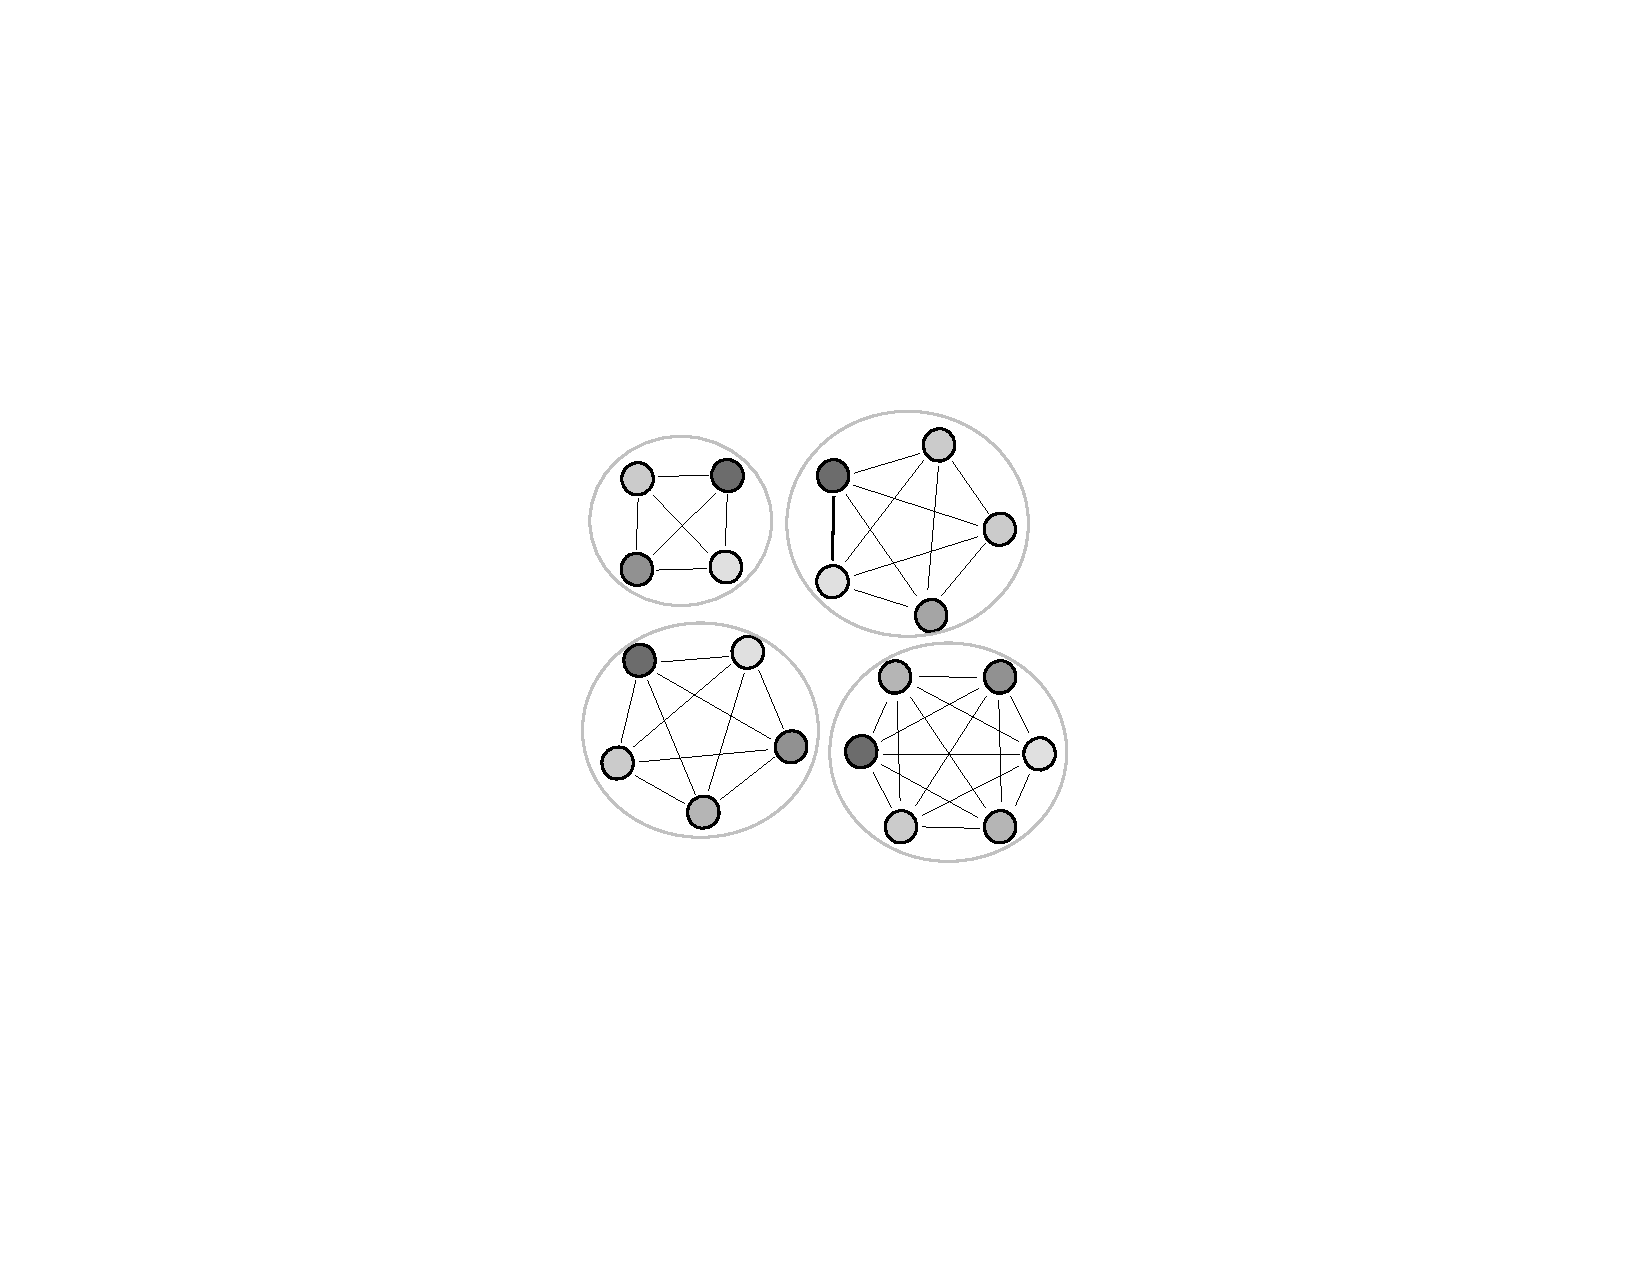
\includegraphics[scale=0.3]{figures/Contrast_circle}
        \caption{Contrastive}
        \label{fig:contrastive}
    \end{subfigure}%
    \begin{subfigure}{0.25\textwidth}
        \centering
        %\includegraphics[width=\linewidth,height=5cm]{figures/drawing}
            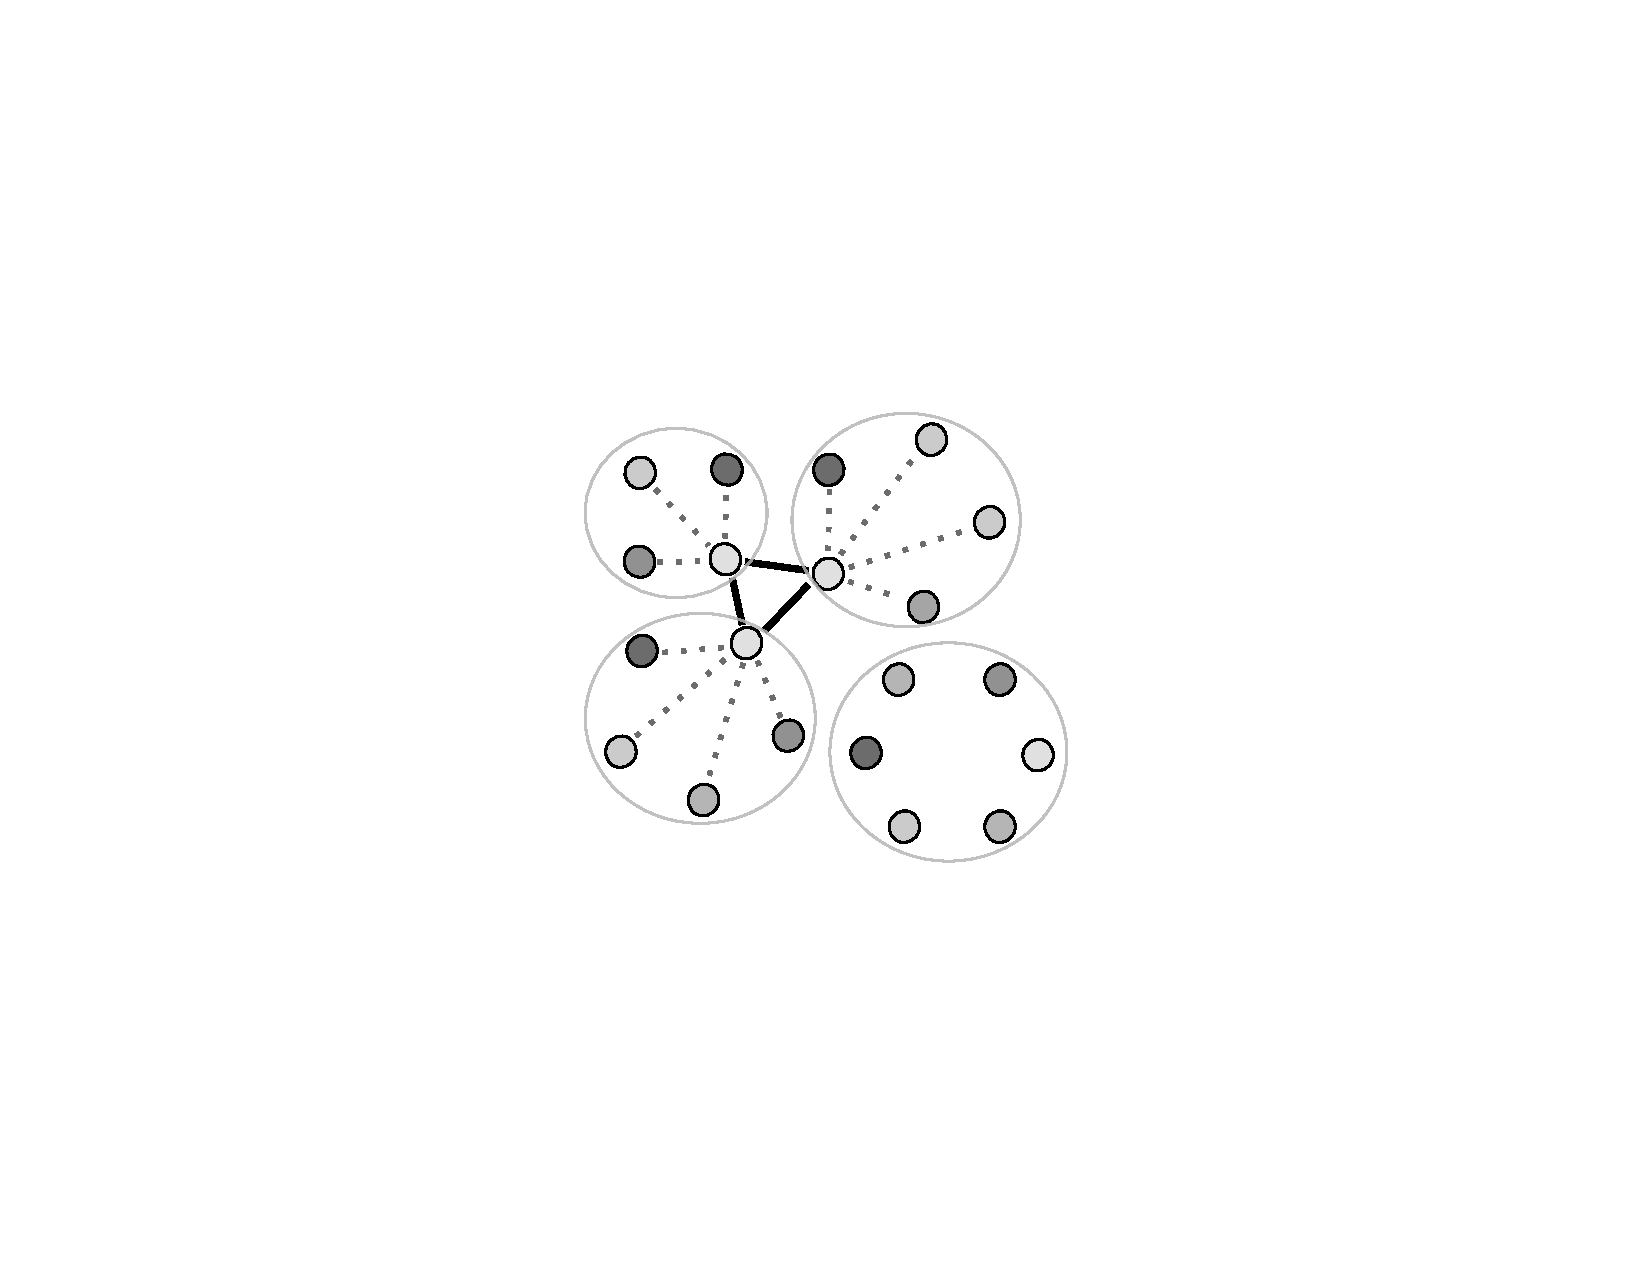
\includegraphics[scale=0.3]{figures/similarContrast_old}
      \caption{Similarity by Contrast}
      \label{fig:similar}
        \end{subfigure}%
        % \begin{subfigure}{0.45\linewidth}
        %     \centering
        %     %\includegraphics[width=\linewidth,height=5cm]{figures/drawing}
        %     \includegraphics[scale=0.275]{figures/Similarity2}
        % \end{subfigure}
        % \caption{TrueSkill / Arrival Similarity}
    %\end{subfigure}%
  %      \caption{\small \label{fig:relation} Induced data-driven relational classes; Contrastive, Relative Similarity and Reflexive among $(q,a)$ tuples. Contrastive relation exists between all answers to a question; Relative Similarity connects answers across questions if relative difference in author's skill with other answerers in each question are significant. Reflexive assumes no dependence on other answers for prediction. }
    \caption{\small \label{fig:relation} Reflexive(~\cref{fig:reflexive}), Contrastive (~\cref{fig:contrastive}) and Similarity by Contrast (~\cref{fig:similar}) relations among $(q,a)$ tuples. Reflexive assumes no dependence on other answers for prediction. Contrastive compares all answers to a question;  Similarity by Contrast connects answers across questions if they differ from other answers similarly. Solid lines indicate similarity, while dotted lines indicate contrast. The contrast is only significant in three questions in the above example.}
    \vspace{-0.15in}
\end{figure*}

%In this section, we define and operationalize the three class of \emph{induced relational views} among the $(q, a)$ tuples introduced above. Each $(q,a)$ tuple constitutes a node in each induced relational view of the dataset. We now describe the precise construction of the links in each view. We aim to facilitate feature sharing (with similarity views) and feature discrimination (with contrastive views) among linked nodes.

%In this section, we define and operationalize the  %Each $(q,a)$ tuple constitutes a node in each induced relational graph of the dataset.
% In this section, we describe the construction of the views representing three different strategies. %We induce these relational views across $(q,a)$ tuples with differing criteria (hence \textit{induced relational views}).

% Our views are designed to achieve feature sharing for the \emph{relative similarity} strategy, feature comparison for the \emph{contrastive} strategy and feature evaluation for the \emph{reflexive} strategy.

%As we observed in the previous section, we formulate answer selection as a node classification problem to facilitate explicit feature sharing (in case of similarity views) and feature discrimination (in case of contrast views) across nodes based on the induced links in each view.

% \begin{wrapfigure}{R}{0.15\textwidth}
% \centering
% \includegraphics[height=3cm,width=0.1\textwidth]{figures/example_human}
% \caption{\small \label{fig:contrast}Contrastive Relation}
% \end{wrapfigure}

%
% \begin{figure}[h]
%     \centering
%     %\includegraphics[height=4cm,width=0.45\textwidth]{figures/clique_size_distribution}
%     \includegraphics[scale=0.15]{figures/clique_size_distribution}
%     \caption{\small \label{fig:clique_size_dist} Distribution of clique sizes for Contrastive relation (i.e. number of answer per question) in StackExchange communities. It follows a long tail distribution with higher variance across communities for large clique sizes.}
%     %\vspace{-0.1in}
% \end{figure}

\subsection{Constructing Induced Views}
\label{sub:Induced Views}


In this section, we discuss four sample strategies that represent strategies to label an answer as `accepted.' Each strategy $S_i \in \mathbf{S}$ \textit{induces} a graph $G_i = (V, E_i)$ (also referred to as a relational view). In each graph $G_i$, a vertex $v \in V$ represents a tuple $(q,a)$ and an edge $e \in E_i, E_i \subseteq V \times V$ connects two tuples that are related under that strategy or view. Note that each $G_i$ has the same vertex set, while edge sets $E_i$ depend on strategy $S_i$. Each strategy employs one of the three different relation types, reflexive, contrastive, and similarity to connect the tuples. We use one reflexive strategy, one contrastive, and two similarity strategies in our experiments. \Cref{fig:relation} summarizes the three relations. We organize the below discussion by relation type.

%In each case, the vertex set $V$ is the same across the different $G_i$, and the edge sets $E_i$ are strategy dependent.
%Each strategy use three different relations between nodes and their corresponding graphs.
%Now we discuss in detail four example strategies that can be used to identify answers that the individual posting the question will label as `accepted'in CQA forums.
%the construction of a graph $G_i = (V, E_i)$ , corresponding to each of the $i=4$ different strategies.
%class of relational views
% \noindent

\subsubsection{Reflexive}
\label{sub:Reflexive}

A natural strategy is to examine each $(q,a)$ tuple in isolation and then assign a label $y_{q,a} \in \{-1,+1 \}$ corresponding to `not accepted' or `accepted.' In this case, $y_{q,a}$ depends on only the features of $(q,a)$. This is a \textbf{Reflexive} relation, and the corresponding graph $G_r = (V,E_r)$ has a specific structure. In particular, in this graph $G_r$, we have only self-loops, and all edges $e \in E_r$ are of the type $(v,v)$. That is, for each vertex $v \in V$, there are no edges $(v,u)$ to any other vertices $u\neq v \in V$. Much of the prior work on feature driven answer selection~\cite{BurelMA16,JendersKN16,TianZL13,TianL16} adopts this view.

\subsubsection{Contrastive}
\label{sub:Contrastive}

A second strategy is to examine answers \textit{in relation} to other answers to the same question and label one such answer as `accepted.' Thus the second strategy \textit{contrasts} $(q,a)$, with other tuples in  $(q,a'), q \in \mathcal{Q}; a, a' \in \mathcal{A}_q; a'\neq a$. This is a \textbf{Contrastive} relation and the corresponding graph $G_c = (V,E_c)$ has a specific structure. Specifically, we define an edge $e \in E_c$ for all $(q,a)$ tuples for the same question $q \in \mathcal{Q}$. That is, if  $v = (q_1, a_1), u=(q_2, a_2)$, $e=(u, v) \in E_c \iff q_1=q_2$. Intuitively, the contrastive relation induces cliques connecting all answers to the same question. Introducing contrasts between vertices sharpens differences between features, an effect (described in more detail in~\Cref{subsec:contrast}) we term \emph{Discriminative Feature Magnification}. Notice that the contrastive relation is distinct from graphs with signed edges (e.g.,~\cite{signedgcn}). In our framework, the contrast is a \textit{neighborhood} property of a vertex, whereas in~\cite{signedgcn}, the negative sign is a property of an \textit{edge}.


% The \textbf{Contrastive} strategy discriminates the features of accepted answers against their competitors. %We propose a specific operationalization of the contrast view drawing upon the tournament view of each question in the forum.
% %\textbf{Tournament-Style Contrast:}
% Thus, we construct links between tuples $(q, a)$ and $(q, a')$ for questions $q \in Q$ and their answers $\texttt{ }\forall \texttt{ } a,a' \in \mathcal{A}_q$ under this view.
% %For questions $q \in Q$, and their answers $\mathcal{A}_q$, we construct links between tuples $(q, a)$ and $(q, a')  \texttt{ }\forall \texttt{ } a,a' \in \mathcal{A}_q$ resulting in a clique of answers to each question.
% The resulting view is a disconnected collection of cliques of answers to each question with size equal to $\lvert\mathcal{A}_q\rvert$ (~\cref{fig:relation}). Note that in each clique, one answer has an accepted label while the rest do not.
% %(the distribution of clique sizes for StackExchange communities is indicated in \cref{fig:clique_size_dist}).
% % The motive of these induced links is better described in \cref{sec:model} where we discuss Induced Relational Graph Convolution to enable feature sharing across vertices for classification in each induced view.
% The connections across accepted and non-accepted answers to a question enable feature contrast. We design our convolutional model to magnify and encode these differences in \cref{subsec:contrast}, an effect we term \emph{Discriminative Feature Magnification}.
% %The set of cliques can thus be given by $\mathbf{C}_q$ consisting of the links between every $(q,a)$ tuple, where the question is $q$ and $a \in \mathcal{A}_q$.

% %The \textbf{Contrastive} view is induced between all competing players in a specific tournament (i.e., competing answers to a question) and captures the disparity between the accepted $(q,a)$ tuples and the rest of the competing answers to a question. The primary objective of contrast  All the $(q, a)$ tuples of a single question is connected to capture feature contrast through an effect we call \textbf{Discriminative Magnification}. We describe this effect in greater detail in the section Our operationalization of the view is as follows:


\subsubsection{Similarity by Contrast}
\label{sub:Similar}
A third strategy is to identify \textit{similar} $(q,a)$ tuples \textit{across} questions. Prior work~\cite{Wu2016} indicates that individuals on StackExchange use diverse strategies to contribute answers. Experts (with a high reputation) tend to answer harder questions, while new members (with low reputation)  looking to acquire reputation tend to be the first to answer a question.

How might similarity by contrast work? Consider two individuals Alice and Bob with \textit{similar} reputations (either high or low) on StackExchange, who contribute answers $a_A$ and $a_B$ to questions $q_1$ and $q_2$ respectively. If Alice and Bob have high reputation difference with other individuals who answer questions $q_1$ and $q_2$ respectively, then it is likely that $(q_1, a_A)$ and $(q_2, a_B)$ will share the same label (if they are both experts, their answers might be accepted, if they are both novices, then this is less likely). However, if Alice has a high reputation difference with other peers who answer $q_1$, \textit{but Bob does not have that difference} with peers who answer $q_2$, then it is less likely that the tuples $(q_1, a_A)$ and $(q_2, a_B)$ will share the label, even though the reputations of Alice and Bob are similar.

Thus the key idea of the \textbf{Similarity by Contrast} relation is that link tuples that are  \textit{similar in how they differ} with other tuples. We construct the graph $G_s = (V, E_s)$ in the following manner. An edge $e = (v,u)$ between tuples $v$ and $u$ exists if the similarity $s(v,u)$ between tuples $v,u$ exceeds a threshold $\delta$. We define the similarity function $s(\cdot , \cdot)$ to encode similarity by contrast. That is, $e=(v,u) \in E_s \iff s(v,u) \geq \delta$.

% \begin{figure}[htbp]
%   \centering
%   \begin{subfigure}{0.23\textwidth}
%     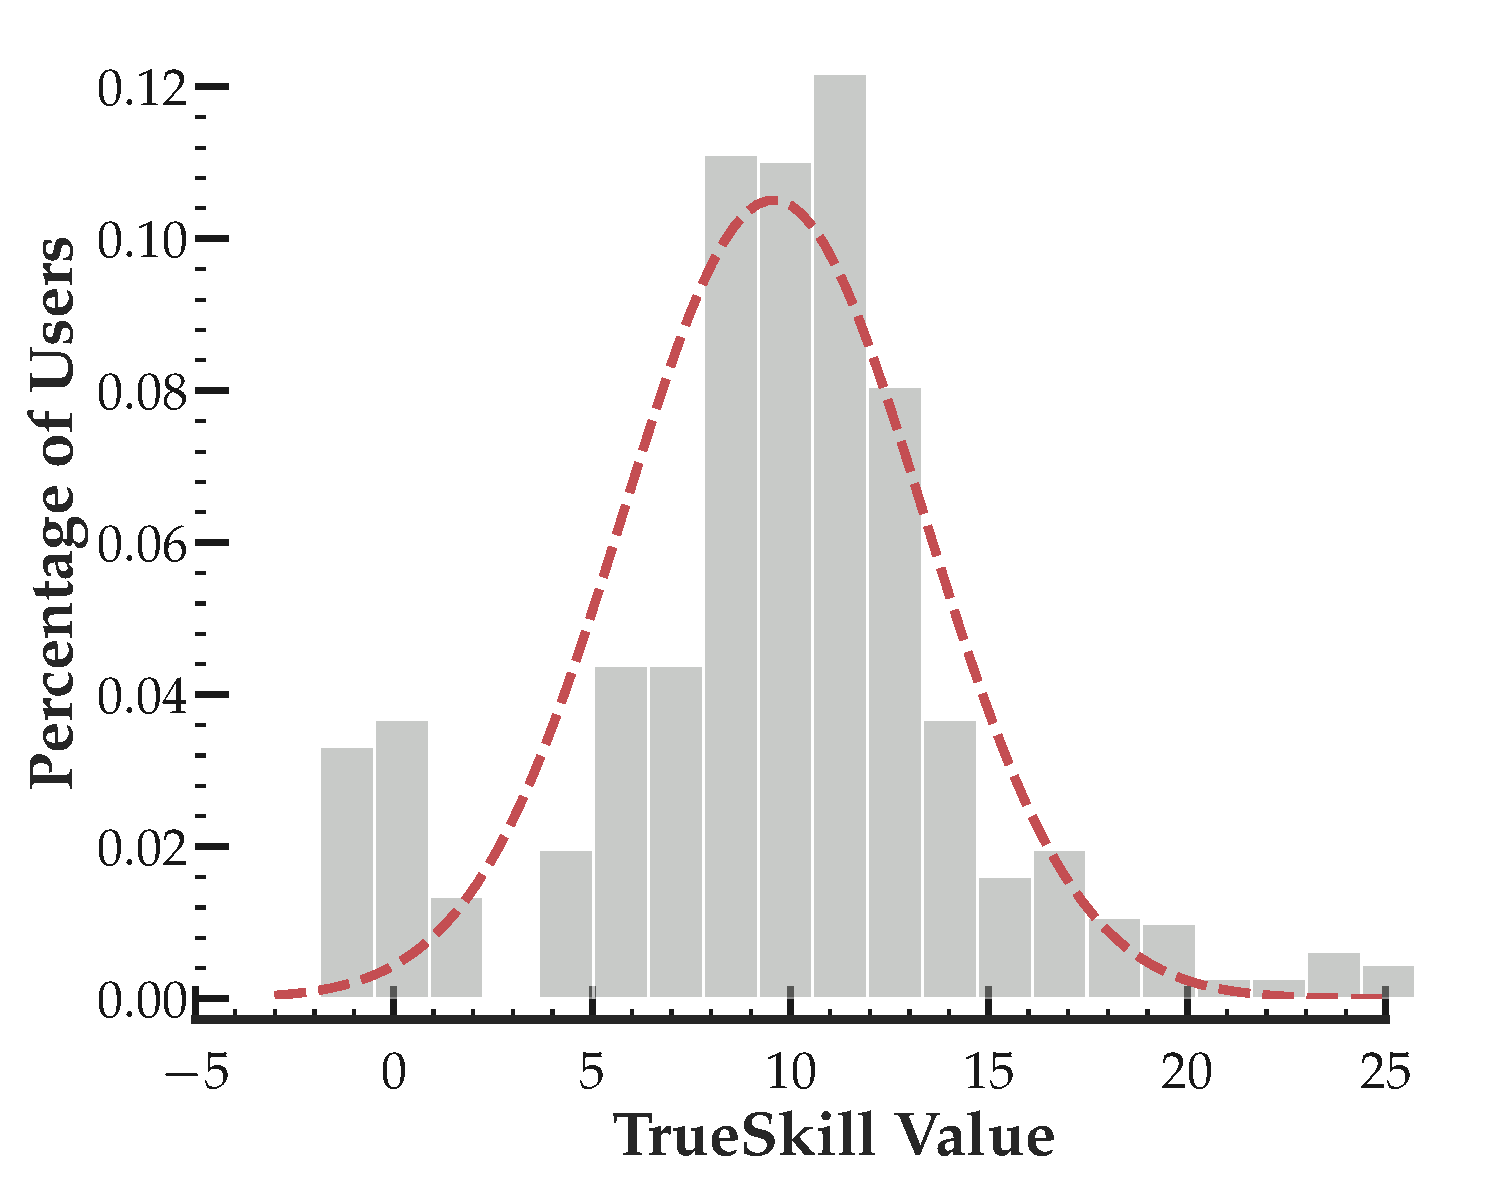
\includegraphics[height=3cm,width=\textwidth]{figures/TrueSkill}
%     \caption{TrueSkill Distribution}
%   \end{subfigure}%
%   \begin{subfigure}{0.23\textwidth}
%     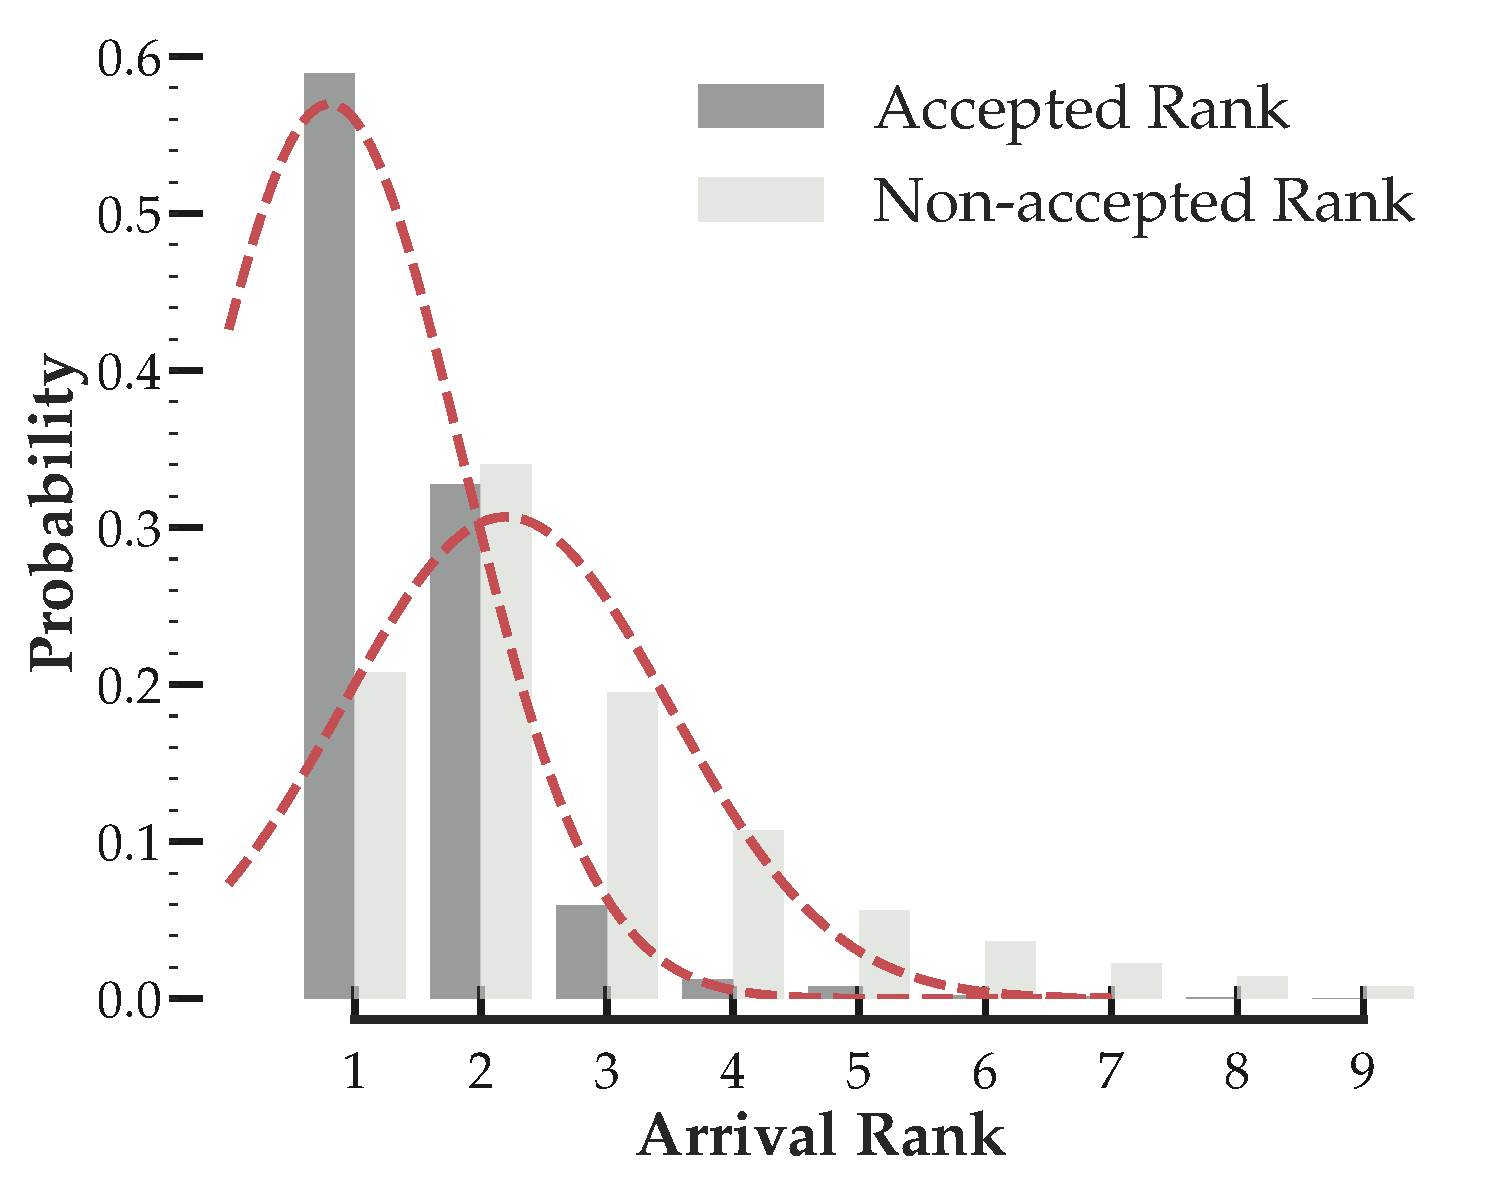
\includegraphics[height=3cm,width=\textwidth]{figures/ArrivalRank}
%     \caption{ArrivalRank Distribution}
%   \end{subfigure}
%   \caption{\small \label{fig:similarcontrastsempirical} Distribution of the TrueSkill values of users and ArrivalRank of accepted answers and non-accepted answers for the movie StackExchange. Early answers are more likely to be accepted and variance of TrueSkill similarity across users is high.}
% \end{figure}

Motivated by~\cite{Wu2016}, we consider two different views that correspond to the similar contrast relation. The \textbf{TrueSkill Similarity} view connects all answers authored by a user where her skill (computed via Bayesian TrueSkill~\cite{TrueSkill06})) differs from competitors by margin $\delta$. We capture both cases when the user is less or more skilled than her competitors. In the \textbf{Arrival Similarity} view, we connect answers across questions based on the similarity in the relative time of their arrival (posting timestamp).
% ~\Cref{fig:similarcontrastsempirical} shows the distribution of skill and the relationship of answer acceptance to arrival rank in StackExchange. We see a wide skill distribution and that the earlier answer has a higher probability of acceptance.
Notice that two Similarity by Contrast views have different edge ($E$) sets since the corresponding similarity functions are different. Notice also, that the two similarity function definitions are transitive.
%%%%%%%INCLUDE COAUTHOR REASON
 \footnote{One trivial way of establishing similarity is co-authorship i.e. connect all $(q,a)$ tuples of a user (probably on the same topic) across different questions.
%Thus, we can connect each $(q,a)$ and $(q',a'); q,q' \in \mathcal{Q}, a \in \mathcal{A}_q, a' \in \mathcal{A}_q'$ such that $u_a = u_{a'}$.
Note that the accepted answer is labeled relative to the other answers. As the competing answers are different in each question, we can not trivially assume acceptance label similarity for all co-authored answers. In our experiments, co-authorship introduced a lot of noisy links in the graph leading to worse performance.}

\subsection{Generalized Views}
\label{sub:Generalized Views}
Now we present the general case of the induced view. First, notice that each of the three relation types that we consider---reflexive, contrastive, and similarity---result in a graph $G_i = (V, E_i)$ comprising a set of cliques. This is not surprising, since all three relations presented here, are equivalence relations. Second, observe the semantics of how we select the tuple with the accepted answer. Within the three relations, we used two semantically different ways to assign the `accepted' answer label to a tuple. One way is to share the labels amongst all the vertices in the \textit{same clique} (used in the reflexive and the similarity relations). The second is to \textit{assign label based on contrasts with other vertices} in the same clique. We can now state the organizing principle of our approach as follows.
\begin{quote}
  A generalized \textit{modular} framework: pick a meaningful equivalence relation on the $(q,a)$ tuples to induce graph comprising cliques and then apply specific label semantics (label sharing or label contrast) within each clique.
\end{quote}

Equivalence relation results in a graph with a set of disconnected cliques. %Then, within a clique, one could use application-specific semantics, different from two discussed in this paper, to label tuples as `accepted.'
%For example, we could restrict the determination of label via contrast to tuples that satisfy some criteria (e.g., gender, location, education, etc.).
Cliques have some advantages: they have well-defined graph spectra~\cite[p. 6]{Chung1997}; cliques allow for \textit{exact} graph convolution; parallelize the training as the convolution of a clique is independent of other cliques.
%parallelize training and testing.

%Thus, each strategy induces a graph $G_i=(V,E_i)$ using one of the three equivalence relations---reflexive, contrastive, and similarity---and then applies one of the two semantics (`share the same label'; `determine label based on contrast').
% While the modular separation between graph construction and label semantics does not imply that we construct the graph (or the view) $G$ via an equivalence relations,


% Cliques have well defined graph spectra~\cite{Chung1997} and may speed up Graph Convolution Networks (GCNs) by running the convolution in parallel across cliques.

% Thus, our induced view framework readily generalizes to admit \textit{any} equivalence relation. Equivalence partitions of vertices in $G$ result in cliques. Then, within a clique, one could use application specific semantics to label tuples as `accepted.' For example, we could also consider alternate semantics such as `label at most two answers as `accepted'' etc. Cliques have well defined graph spectra~\cite{Chung1997} and may potentially speed up Graph Convolution Networks (GCNs) by running the convolution in parallel across cliques.




% we next discuss induced relational GCNs.

% and then applies a specific semantic (`contrast'; `similar').

%Thus far, we've discussed $i=4$ strategies, and their corresponding views or graphs $G_i = (V, E_i)$. Each strategy used one of the three equivalence relations---reflexive, contrast, similar---resulting in $G_i$ being a set of cliques. We introduced two label selection mechanisms (`share labels within a clique', `assign label by contrast'), and in the next section we show how to make operational these mechanisms on a view $G_i$ via a graph convolution.
% equivalence relations---reflexive, contrastive and similar---and the corresponding graphs $G_k = (V,E_k)$ along with two different

% provides a temporal metric against competitors. The temporal arrival patterns of answers are correlated to their acceptance probabilities (\cref{fig:clique}). For a specific user authoring answers $a, a'$ to questions $q, q'$, we establish a link between $(q,a)$ and $(q',a')$ if %$\lvert T_{a} - T_{b} \rvert > \gamma \times \max(T_{b}); \forall b \in \mathcal{A}_(q)$ and $\lvert T_{a'} - T_{c} \rvert > \gamma \times \max(T_{c}); \forall c \in \mathcal{A}_(q')$.
% %Highly skilled/active users tend to follow consistent patterns in when they author answers, relative to the other competing answers.
% %We observe that earlier posted answers have a higher chance of acceptance in CQA platform as shown in Figure \ref{fig:clique}. Therefore,
% \begin{align*}
%  \lvert T_{a} - T_{b} \rvert &> \gamma \times \max(T_{b}), \hspace{3pt} \forall b \in \mathcal{A}_(q), b \neq a \hspace{5pt} \textsc{AND} \\
%  \lvert T_{a'} - T_{c} \rvert &> \gamma \times \max(T_{c}), \hspace{3pt} \forall c \in \mathcal{A}_(q'), c \neq a'
% \end{align*}
% where $T_{a}$ represents the number of seconds between the question and answer $a$. Hence we connect answers that are quicker or slower than their competitors by a $\gamma$ factor.


% Specifically, if the user authors answers $a, a'$ to questions $q, q'$, we connect tuples $(q,a)$ and $(q',a')$ where %$\lvert S_{u_a} - S_{u_b} \rvert > \delta; \forall b \in \mathcal{A}_(q)$ and $\lvert S_{u_a'} - S_{u_c} \rvert > \delta; \forall c \in \mathcal{A}_(q')$
% \begin{align*}
%  \lvert \textit{TS}_{u_a} - \textit{TS}_{u_b} \rvert &> \delta, \hspace{3pt} \forall b \in \mathcal{A}_(q), b \neq a  \hspace{5pt} \textsc{AND}\\
%  \lvert \textit{TS}_{u_{a'}} - \textit{TS}_{u_c} \rvert &> \delta, \hspace{3pt} \forall c \in \mathcal{A}_(q'), c \neq a'
% \end{align*}
% where $\textit{TS}_{u_a}$ is the skill value for the user who authored answer $a$ (we estimate user skill values with TrueSkill rating \cite{TrueSkill06}). This captures both cases, i.e. where the user is less or more skilled than his competitors.







% For example, answers by individuals with low reputation are likely not `accepted' for a question if there is also an answer by an individual with high reputation to the same question. Thus two tuples $(q,a), q \in \mathcal{Q}, a \in \mathcal{A}_q$ and $(q',a'), q' \in \mathcal{Q}, a \in \mathcal{A}_{q'}$ by (possibly different) low-reputation individuals are \textit{similar in how they differ} with other tuples corresponding to the same questions $q$ and $q'$ respectively.


% \textbf{Reflexive} strategy evaluate $(q, a)$ tuples in isolation as illustrated in \cref{fig:relation}. In such cases, the label prediction for $(q, a)$ tuple depends on it's features alone. This view encompasses most feature-driven answer selection methodology~\cite{BurelMA16,  JendersKN16, TianZL13, TianL16}.





% \noindent
% The \textbf{Similarity} \emph{by contrast} strategy connects answers across different questions by relative comparison against their competitors. Consider a simplified example (~\cref{fig:relation}); user Alice answers four questions with varying numbers of competing answers. Assume a wide skill-margin between Alice and the authors of the other answers in three questions. In these three cases, it is likely that her answer is accepted or the converse depending on her relative skill. However, results are uncertain in scenarios where the author skill differences are not as pronounced. The relative similarity of Alice's answers (high skill margins) to competing answers enables us to make a confident prediction. Hence, one way to create a \emph{similarity by contrast} view is by author skill. We create two diverse similarity by contrast views in our experiments:%In a more general sense, this is true of other answer features as well.

%Therefore, tournament outcomes are likely to be similar when answers are authored by users who differ from those of competing answers by significant margins. There are two such cases, the user has a significantly greater skill than the competing authors, and the opposite case. The intermediate cases are more uncertain. The resulting graph is again a complete graph as all such $(q, a)$ pairs are connected to each other.

 %By employing author skill as a proxy, we are able to learn the associations of other answer features to the acceptance outcome.


% The \textbf{TrueSkill Similarity} view connects all the answers authored by a user where his skill differs from competitors by margin $\delta$. Specifically, if the user authors answers $a, a'$ to questions $q, q'$, we connect tuples $(q,a)$ and $(q',a')$ where %$\lvert S_{u_a} - S_{u_b} \rvert > \delta; \forall b \in \mathcal{A}_(q)$ and $\lvert S_{u_a'} - S_{u_c} \rvert > \delta; \forall c \in \mathcal{A}_(q')$
% \begin{align*}
%  \lvert \textit{TS}_{u_a} - \textit{TS}_{u_b} \rvert &> \delta, \hspace{3pt} \forall b \in \mathcal{A}_(q), b \neq a  \hspace{5pt} \textsc{AND}\\
%  \lvert \textit{TS}_{u_{a'}} - \textit{TS}_{u_c} \rvert &> \delta, \hspace{3pt} \forall c \in \mathcal{A}_(q'), c \neq a'
% \end{align*}
% where $\textit{TS}_{u_a}$ is the skill value for the user who authored answer $a$ (we estimate user skill values with TrueSkill rating \cite{TrueSkill06}). This captures both cases, i.e. where the user is less or more skilled than his competitors.
%\begin{align*}
% \lvert S_{u,a} - S_{u, b} \rvert < -\delta; \forall b \in \mathcal{A}(q) \\
% \lvert S_{u,a'} - S_{u, c} \rvert < -\delta; \forall c \in \mathcal{A}(q')
%\end{align*}
%TrueSkill values are normally distributed among users (\cref{fig:clique}).

% developed by Microsoft Reasearch for ranking and matching similar skill game players for Xbox Live. In our settings, each question is a multi player game with all answerers as game players. The user who gives credible answer is the winner. True Skill rating then computes player's skill through bayesian inference on the basis of credibility label of his answered questions. The estimated ratings are a Gaussian distribution where $\mu$ denotes the average skill of the player. We use the mean value as skill value for our computations.

%Therefore, each user can have at most two cliques, one which connects all his answers where his true skill is significantly better than other answerers of the question; and second where his skill is vastly lower than all the other answerers. In the first case, he is highly likely to give accepted answers while in other his answer would be classified as non-accepted. As CQA platforms encompass variety of topics, each user can be accepted in one topic while non accepted for other topics in the same community.

% Formally, output of the $i$-th hidden layer for True Skill Similarity GCN network $Z_{ts}^{(k)}$ is defined as:
% \begin{equation}
%   \label{eq:TSsimilarity}
%   Z_{ts}^{k} = \sigma\left((I_N + D^{-\frac{1}{2}}A_{ts}D^{\frac{1}{2}}) Z_{ts}^{(k-1)}W_s^{(k)} \right)
% \end{equation}
% with $A_{ts}$ being the adjacency matrix for true skill similarity relations.


% \textbf{Arrival Similarity} view provides a temporal metric against competitors. The temporal arrival patterns of answers are correlated to their acceptance probabilities (\cref{fig:clique}). For a specific user authoring answers $a, a'$ to questions $q, q'$, we establish a link between $(q,a)$ and $(q',a')$ if %$\lvert T_{a} - T_{b} \rvert > \gamma \times \max(T_{b}); \forall b \in \mathcal{A}_(q)$ and $\lvert T_{a'} - T_{c} \rvert > \gamma \times \max(T_{c}); \forall c \in \mathcal{A}_(q')$.
% %Highly skilled/active users tend to follow consistent patterns in when they author answers, relative to the other competing answers.
% %We observe that earlier posted answers have a higher chance of acceptance in CQA platform as shown in Figure \ref{fig:clique}. Therefore,
% \begin{align*}
%  \lvert T_{a} - T_{b} \rvert &> \gamma \times \max(T_{b}), \hspace{3pt} \forall b \in \mathcal{A}_(q), b \neq a \hspace{5pt} \textsc{AND} \\
%  \lvert T_{a'} - T_{c} \rvert &> \gamma \times \max(T_{c}), \hspace{3pt} \forall c \in \mathcal{A}_(q'), c \neq a'
% \end{align*}
% where $T_{a}$ represents the number of seconds between the question and answer $a$. Hence we connect answers that are quicker or slower than their competitors by a $\gamma$ factor.
%\begin{align*}
% \lvert T_{a} - T_{b} \rvert < -\gamma * max(T_{b}); \forall b \in \mathcal{A}(q) \\
% \lvert T_{a'} - T_{c} \rvert < -\gamma * max(T_{c}); \forall c \in \mathcal{A}(q')
%\end{align*}
% Our hypothesis is that a similar answering schedule is correlated with acceptance probabilities.

%\begin{comment}
%is based on similarity in the difference of arrival time of answers for a question.
%Consider this hypothetical example, for $q$, the timestamp(minutes) of the difference in answers' arrivals with respect to question's post timestamp are listed below:\\
%$a_1$: 10 \\
%$a_2$: 10000 \\
%$a_3$: 10100 \\
%$a_4$: 10110 \\
%There is higher likelihood of $a_1$ being judged the credible answer as it occured 10 minutes of posting the question. CQA platforms are used for quick discussions and answers posted much later, although could be correct, have much lower likelihood of being accepted. Also note that, for StackExchange, questioner can not change their accepted answer at a later time.
%While for Q2, the timestamp(minutes) of the difference in answers' arrivals to the timestamp of question's posting are:\\
%$a_1$: 10 \\
%$a_2$: 11 \\
%$a_3$: 12 \\
%$a_4$: 1000000 \\
%which means $a_4$ is highly probable not to be accepted.
%\end{comment}

%Thus, for each user, we construct a clique of all answers in which she answers significantly earlier than other answers, and another clique with all answers in which her answer is much later than all other answers for that question.

%
% Formally, output of the $k$-th hidden layer for Arrival Similarity GCN network $Z_{as}^{(k)}$ is defined as:
% \begin{equation}
%   \label{eq:ASsimilarity}
%    Z_{as}^{k} = \sigma \left((I_N + D^{-\frac{1}{2}}A_{as}D^{\frac{1}{2}}) Z_{as}^{(k-1)}W_s^{(k)} \right)
% \end{equation}
% with $A_{as}$ being the adjacency matrix for arrival similarity relationship.




%As noted before, answer selection is a relational property. Thus standard similarity relationships among users of similar skills do not help label prediction. For instance, in the given example, even if Alice has good ratings, she has to be better in \emph{relative} to all other players in the tournament.


% \begin{wrapfigure}{R}{0.15\textwidth}
% \centering
% \includegraphics[height=1.85cm,width=0.1\textwidth]{figures/Reflexive_v2}
% \caption{\small \label{fig:reflex}Reflexive Relation}
% \end{wrapfigure}
%\paragraph{}
%\vspace*{-\parskip}



% Secondly, the tournament-style contrast view is deterministic, we can precisely determine the set of competing answers to a given question (or tournament). On the other hand, relative similarity can be operationalized in many ways (TrueSkill and Arrival Similarity are two relevant views in CQA) and the induced links are inherently noisy. This is a key factor to consider when we develop our node classification architecture in the next section.

%In contrast to Ts. In this paper, we propose an automated graph construction mechanism using data driven induced relationships with minimal human supervision. The graph construction is based on certain user defined criterions which are domain dependent and can be easily adapted to other domains. Note that this is a generic framework and we can introduce other higher-order relationships (like triangles) for different domains.


% Finally, \textbf{Reflexive} strategy evaluate $(q, a)$ tuples in isolation as illustrated in \cref{fig:relation}. In such cases, the label prediction for $(q, a)$ tuple depends on it's features alone. This view encompasses most feature-driven answer selection methodology~\cite{BurelMA16,  JendersKN16, TianZL13, TianL16}.

%This is inherently similar to what current approaches work on. The classification model makes independent prediction and can be representated by a self loop in the graph.
% That is, each node just depends on it's own features and there is no relation to any other node in the graph.
%Knolwedge graphs are widely used in literature \cite{} for understanding graph structured data. Although these graphs support multiple edge types, these edges are manually labeled. Thus, obtaining this edge information can prove to be expensive and restricts scope of these approaches. In this paper, we propose an automated graph construction mechanism using data driven induced relationships with minimal human supervision. The graph construction is based on certain user defined criterions which are domain dependent and can be easily adapted to other domains. Note that this is a generic framework and we can introduce other higher-order relationships (like triangles) for different domains.

%These relationships can be operationalized in different ways and we next explain our interpretation of these relationships for Answer Selection. We further encode these induced relationships using Graph Convolution Networks (GCN).
%\clearpage
